\chapter{Resultat i conclusions finals}
En aquesta secció s'exposaran les conseqüències del desenvolupament del projecte, així com les possibles actualitzacions que es podrien realitzar a aquest, tant a nivell tècnic i com des de un punt de vista subjectiu.
\section{Avaluació i aprenentatge}
\subsection{Problemes i obstacles}
El desenvolupament d'aquest projecte no ha segut exactament lineal, ja que s'han provat i rebutjat una gran varietat de possibles solucions i tecnologies abans d'aplegar al resultat final.
\\[3mm]
El principal obstacle a l'hora de dur a terme el projecte ha segut l'obsolescència i complexitat de les alternatives que ofereix Java per a realitzar interfícies gràfiques. Les llibreries Swing i JavaFX tenen un funcionament i estil visual antiquat, encara que observem moltes aplicacions modernes construïdes amb aquestes ferramentes, tindre un bon resultat amb els coneixements i recursos dels que es disposen per a aquest projecte era una tasca molt complicada.
\\[3mm]
La solució aparentment més senzilla era canviar de llenguatge de programació a algun web i utilitzar HTML i CSS per a crear una interfície atractiva i més escalable. Aquesta idea es rebutja després de fer diverses proves per dos motius:
\begin{enumerate}
    \item La fragilitat i rendiment dels llenguatges web, ja que no compten amb la robustesa que ofereix un compilador, ni altres característiques com la programació orientada a objectes o un fort sistema de tipus, que (en al meva opinió) són molt beneficioses quan s'escriu software. Aquests motius es troben darrere de la creixent popularitat del llenguatge TypeScript i de l'elecció d'aquest per a codificar el frontend.
    \item La voluntat d'utilitzar tecnologies pròpies del cicle de desenvolupament d’aplicacions multiplataforma i la intenció de realitzar un projecte que utilitzara els conceptes que s'han aprés a classe, tractant de diferenciar-lo del que (en al meva opinió) més bé podria ser un projecte del cicle de desenvolupament d’aplicacions web .
\end{enumerate}
Després de formular la pregunta: "Açò com es fa al \textit{món\ real}?" i investigar aquest aspecte, sorgeix la idea de utilitzar el model d'API RESTful, ja que permet combinar el millor de dos mons, la robustesa i fiabilitat dels llenguatges compilats (Java en aquest cas) i la qualitat de les interfícies gràfiques que ofereix la web.
\subsection{Aprenentatge i conceptes nous}
Per a dur a terme aquest projecte s'han utilitzat tecnologies ja vistes a classe, però també algunes noves, per això, ha segut necessari el aprenentatge autodidacta de ferramentes com Spring Boot, Bootstrap, TypeScript, el protocol HTTP, programació reactiva, programació funcional, GitHub avançat o \LaTeX, entre altres.
\section{Proposta de millores}
Encara que el projecte ha complit el seu objectiu principal de desenvolupar una versió digital i multijugador del joc d'escacs, encara hi ha alguns aspectes que queden per implementar o que tenen marge de millora.
\\[3mm]
Han quedat pendents de desenvolupar algunes funcionalitat pròpies del joc d'escacs, com el rellotge, o alguns moviments especials de peces, per exemple l'enroc o la promoció de peons.
\\[3mm]
Des del punt de vista de l'emparellament multijugador, es podria dissenyar un sistema de cues, per a crear partides amb jugadors aleatoris que també estiguen a l'espera.
\\[3mm]
També queda sense resoldre el mode un jugador i, per tant, la introducció d'una intel·ligència artificial capaç de entendre les normes del joc i realitzar moviments al tauler.
\begin{figure}[H]
    \centering
    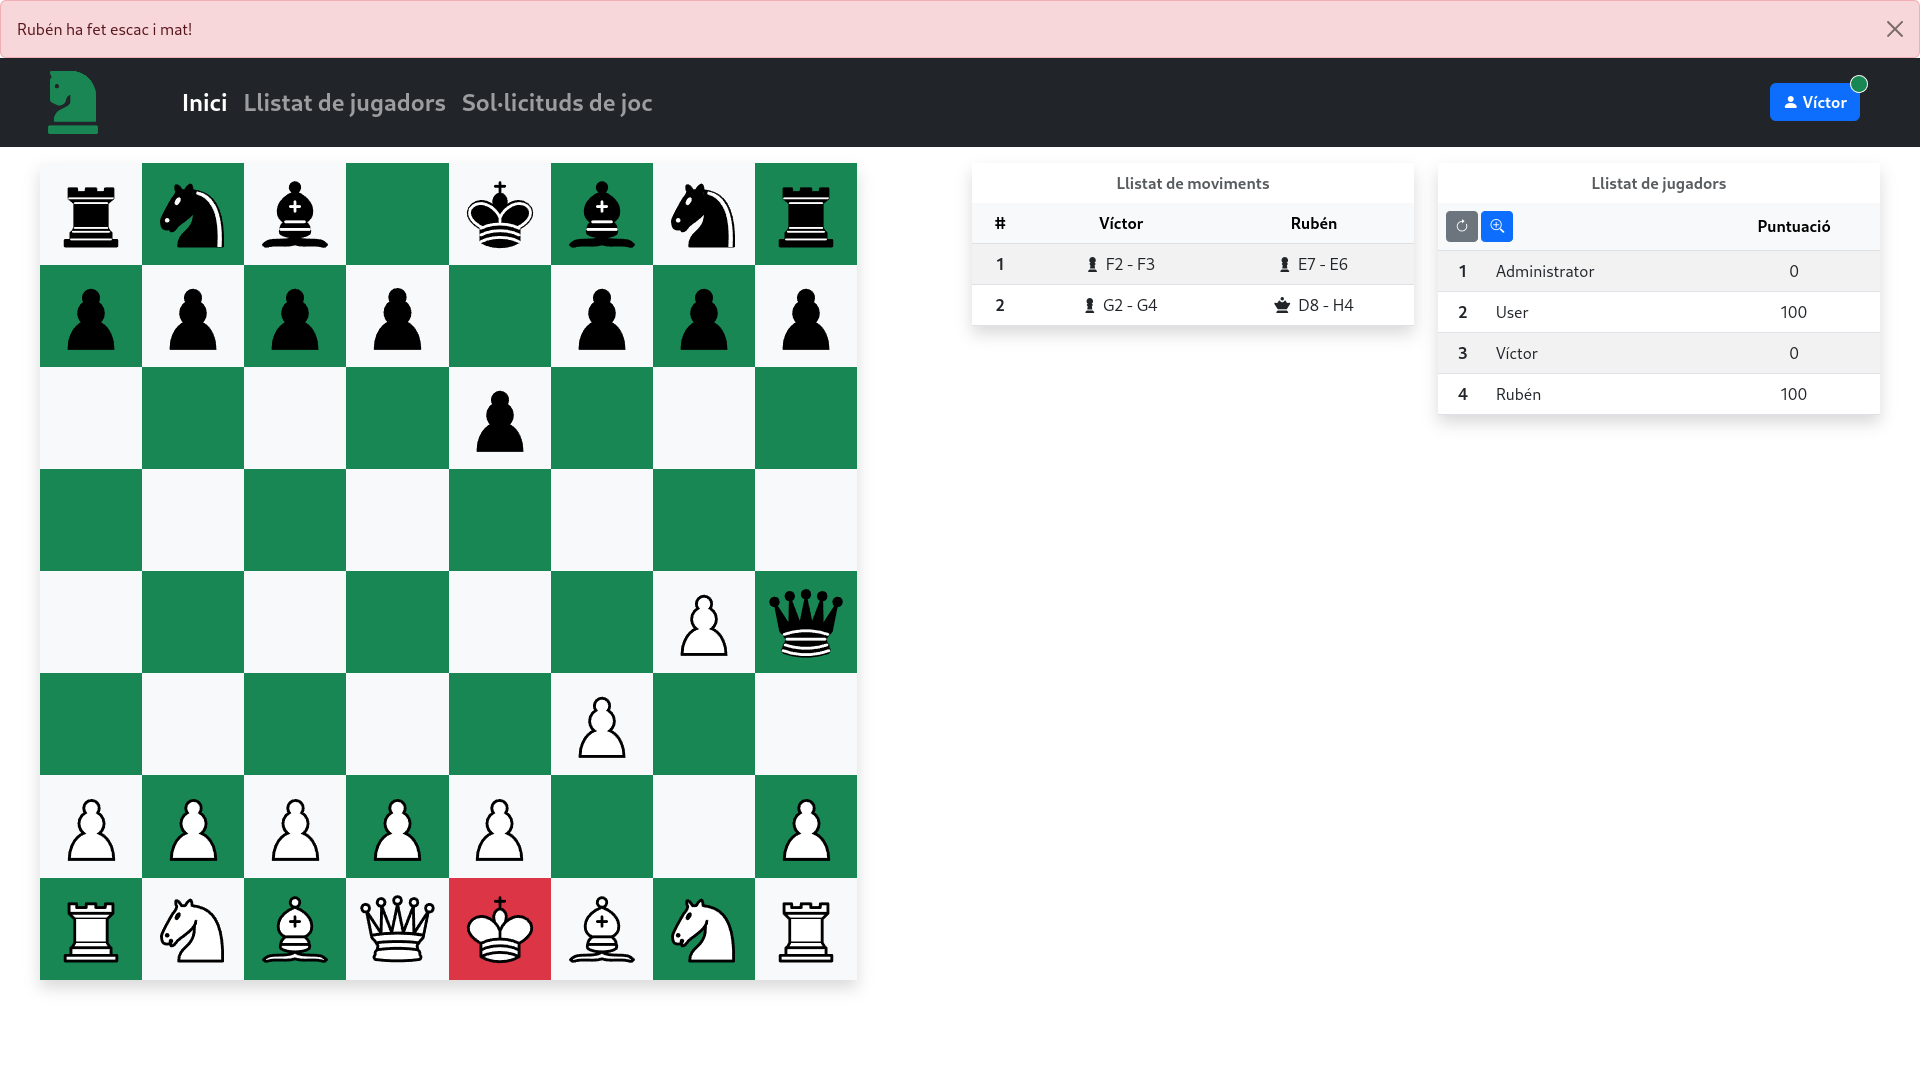
\includegraphics[width=\textwidth]{images/escac-mat.png}
    \caption{Escac i mat}
    \label{fig:Escac i mat}
\end{figure}